% !TeX spellcheck = en_GB
\section{Quality of Iterated Hashing}
\subsection{Implement}
I have implemented both the code for 2a, 2b and 2c. The implementation can be seen in \texttt{src/hash.c} and specifically the calculation of $m(i)$ from $0$ to $1000$ corresponds to the method \texttt{question2\_c(int i)}.

\subsection{Plot}
\begin{figure}[H]
	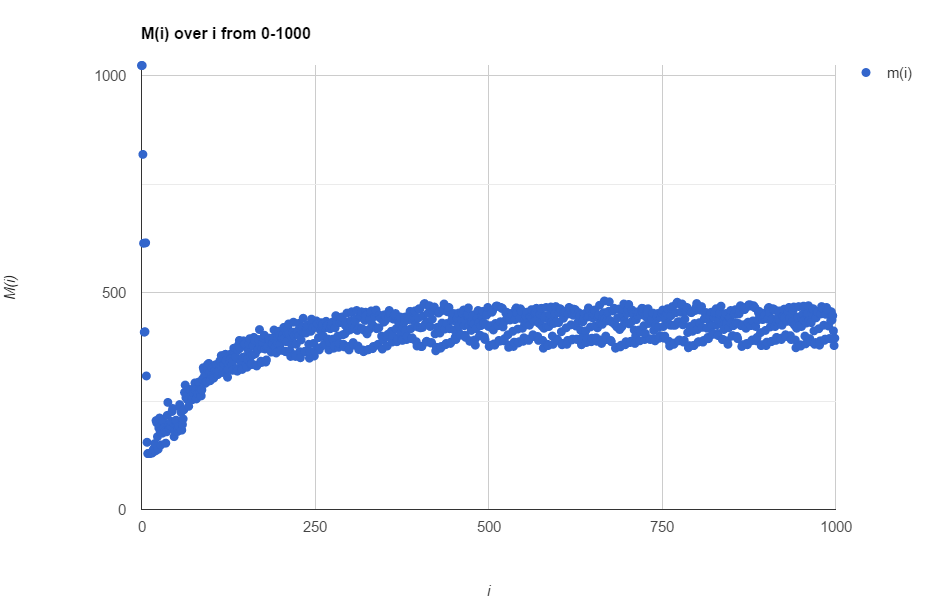
\includegraphics[width=\linewidth]{figures/question2_plot.png}
	\caption{A graph showing the values of m(i) where $i$ ranges from $0...999$}
	\label{graph:question2_plot}
\end{figure}

On figure \ref{graph:question2_plot} the result of running my implementation of $m(i)$ with $i$ from 0 to 1000 can be seen. If the hash function completely evenly distributed the elements then there would be 128 in each bucket. For $i=9,10,11$ $m(i)$ results in $129$, which is very close to an equal distribution. For larger values; $i>300$, $m(i)$ seem to reach a level from around $370$ to $450$, which is approximately a factor of $3.25$ away from the optimal value. 

\subsection{Implementation Question to discuss}
In theory every calculation of m(i) is independent from any other calculation of $m(i+x)$, but because we know that $m(i)$ is related to $m(i-1)$ we achieve a greater speed-up by reusing the answer from the previous calculation than from using multicore parallelization. 

The most obvious loop which could use parallelization is the loop going over the elements in $a$ and hashing and storing them. I do not have such a loop in my code, since i use the same loop for bucket allocation. 

My loop which both calculates rehashing and buckets allocation can still use parallelization. A collection of threads could split the $a$ array between them and calculate their buckets. Of course this has the problem that the threads must synchronize the elements of the bucket between them. Since there is only eight buckets, we could only ever use up to 8 threads and that is if the distribution between the buckets were completely equal.

\newpar It would be possible to vectorize the \texttt{h} method. Especially it should be noted that it uses the bitwise $and$, and the bitwise $or$. These operators are available in Intel intrinsics. Therefore one could calculate the hash on 256 bits of integers at a time, which should in provide a speed boost factor of up to 8.